\documentclass{article}[18pt]
\ProvidesPackage{format}
%Page setup
\usepackage[utf8]{inputenc}
\usepackage[margin=0.7in]{geometry}
\usepackage{parselines} 
\usepackage[english]{babel}
\usepackage{fancyhdr}
\usepackage{titlesec}
\hyphenpenalty=10000

\pagestyle{fancy}
\fancyhf{}
\rhead{Sam Robbins}
\rfoot{Page \thepage}

%Characters
\usepackage{amsmath}
\usepackage{amssymb}
\usepackage{gensymb}
\newcommand{\R}{\mathbb{R}}

%Diagrams
\usepackage{pgfplots}
\usepackage{graphicx}
\usepackage{tabularx}
\usepackage{relsize}
\pgfplotsset{width=10cm,compat=1.9}
\usepackage{float}

%Length Setting
\titlespacing\section{0pt}{14pt plus 4pt minus 2pt}{0pt plus 2pt minus 2pt}
\newlength\tindent
\setlength{\tindent}{\parindent}
\setlength{\parindent}{0pt}
\renewcommand{\indent}{\hspace*{\tindent}}

%Programming Font
\usepackage{courier}
\usepackage{listings}
\usepackage{pxfonts}

%Lists
\usepackage{enumerate}
\usepackage{enumitem}

% Networks Macro
\usepackage{tikz}


% Commands for files converted using pandoc
\providecommand{\tightlist}{%
	\setlength{\itemsep}{0pt}\setlength{\parskip}{0pt}}
\usepackage{hyperref}

% Get nice commands for floor and ceil
\usepackage{mathtools}
\DeclarePairedDelimiter{\ceil}{\lceil}{\rceil}
\DeclarePairedDelimiter{\floor}{\lfloor}{\rfloor}

% Allow itemize to go up to 20 levels deep (just change the number if you need more you madman)
\usepackage{enumitem}
\setlistdepth{20}
\renewlist{itemize}{itemize}{20}

% initially, use dots for all levels
\setlist[itemize]{label=$\cdot$}

% customize the first 3 levels
\setlist[itemize,1]{label=\textbullet}
\setlist[itemize,2]{label=--}
\setlist[itemize,3]{label=*}

% Definition and Important Stuff
% Important stuff
\usepackage[framemethod=TikZ]{mdframed}

\newcounter{theo}[section]\setcounter{theo}{0}
\renewcommand{\thetheo}{\arabic{section}.\arabic{theo}}
\newenvironment{important}[1][]{%
	\refstepcounter{theo}%
	\ifstrempty{#1}%
	{\mdfsetup{%
			frametitle={%
				\tikz[baseline=(current bounding box.east),outer sep=0pt]
				\node[anchor=east,rectangle,fill=red!50]
				{\strut Important};}}
	}%
	{\mdfsetup{%
			frametitle={%
				\tikz[baseline=(current bounding box.east),outer sep=0pt]
				\node[anchor=east,rectangle,fill=red!50]
				{\strut Important:~#1};}}%
	}%
	\mdfsetup{innertopmargin=10pt,linecolor=red!50,%
		linewidth=2pt,topline=true,%
		frametitleaboveskip=\dimexpr-\ht\strutbox\relax
	}
	\begin{mdframed}[]\relax%
		\centering
		}{\end{mdframed}}



\newcounter{lem}[section]\setcounter{lem}{0}
\renewcommand{\thelem}{\arabic{section}.\arabic{lem}}
\newenvironment{defin}[1][]{%
	\refstepcounter{lem}%
	\ifstrempty{#1}%
	{\mdfsetup{%
			frametitle={%
				\tikz[baseline=(current bounding box.east),outer sep=0pt]
				\node[anchor=east,rectangle,fill=blue!20]
				{\strut Definition};}}
	}%
	{\mdfsetup{%
			frametitle={%
				\tikz[baseline=(current bounding box.east),outer sep=0pt]
				\node[anchor=east,rectangle,fill=blue!20]
				{\strut Definition:~#1};}}%
	}%
	\mdfsetup{innertopmargin=10pt,linecolor=blue!20,%
		linewidth=2pt,topline=true,%
		frametitleaboveskip=\dimexpr-\ht\strutbox\relax
	}
	\begin{mdframed}[]\relax%
		\centering
		}{\end{mdframed}}
\lhead{Networks and Systems - Compiler Design}


\begin{document}
\begin{center}
\underline{\huge Semantic Analysis}
\end{center}
\section{Semantic Analysis}
\begin{itemize}
	\item Ensure that the program has a well defined meaning
	\item Verify properties aren't caught during earlier phases e.g.
	\begin{itemize}
		\item Variables are declared before they are used
		\item Expressions have the right types
		\item Number and types of arguments of a procedure call agree with the procedure declaration
	\end{itemize}
	\item To check these properties
	\begin{itemize}
		\item We need to check context conditions imposed by the language specification
		\item They can't be checked by context free grammars
		\item We enhance our grammars: attribute grammars
	\end{itemize}
\end{itemize}
\section{Syntax-Directed Definition}
These additional data needed for these checks are stored as attributes on the nodes of the parse tree, forming an annotated parse tree.\\
\\
An attribute may represent any quantity, e.g. type, string, memory allocation ...
\begin{definition}[Syntax-Directed Definition]
A context free grammar in which:
\begin{itemize}
	\item Every grammar symbol has an associated set of attributes
	\item Every production has an associated set of semantic rules for computing the attribute values
\end{itemize}
\end{definition}
\section{Syntax-directed translation}
\begin{definition}[Syntax-directed translation]
\begin{itemize}
	\item Process an input string x using a syntax-directed definition
	\item First build the parse tree for the string x
	\item For every node N of the parse tree that is labelled by a grammar symbol X denote X.a the attribute a of X at node N
	\item If X is a non-terminal the value of attribute X.a is determined using a semantic rule associated with some production
	\item If X is terminal the value of X.a is determined by the lexical analyser
\end{itemize}
\end{definition}
\section{Types of attributes}
There are two main types of attributes
\begin{definition}[Synthesized attribute]
An attribute whose value at a node N is defined in terms of attributes at the children of N and at N itself
\end{definition}
\begin{definition}[Inherited attribute]
An attribute whose value at node N is defined in terms of attributes at N's parent, at N's siblings and at N itself
\end{definition}
If an attribute a is computed by attributes of parent/siblings and children of N, then add a new inherited attribute b at N and express a as a synthesized attribute (using b)
\section{Evaluation of attributes}
Before we evaluate an attribute at a node we must first evaluate all the attributes upon which its value depends\\
\\
Examples:
\begin{itemize}
	\item Only synthesized attributes (S-attributed SDD)
	\begin{itemize}
		\item Evaluate first the children, then the node itself
		\item All the nodes can be evaluated in any bottom-up order
	\end{itemize}
	\item Only inherited attributes
	\begin{itemize}
		\item Evaluate first the parent and all (needed) attributes of siblings and of itself, then evaluate the node itself
		\item Evaluate the tree in some top-down order
		\item However: never only inherited attributes! (compare terminals vs root)
	\end{itemize}
\end{itemize}
With both synthesized and inherited attributes there is no guarantee that there exists an order to evaluate the attributes of all nodes
\begin{center}
	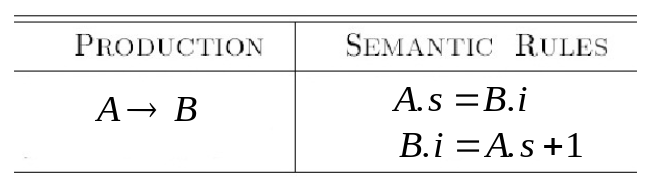
\includegraphics[scale=0.7]{Evaluation_Attributes}
\end{center}
These routes are circular as it is impossible to evaluate either A.s or B.i without first evaluating the other
\section{Dependency Graph}
To check whether there exists an evaluation order for the attributes of an annotated parse tree, we construct the dependency graph\\
\\
A directed graph $G=(N,E)$ with a set of nodes N and a set of directed edges E, with
\begin{itemize}
	\item A node for each attribute in the annotated parse tree
	\item A directed edge $X.c\rightarrow A.b$ whenever in order for compute $A.b$ we have to compute first $X.c$
\end{itemize}
There exists an evaluation order for all the attributes iff the dependency graph has no directed cycles
\newpage
\section{L-attributed SDD}
Some classes of SDD always admit an evaluation order for the attributes
\begin{definition}[S-Attributed SDD]
\begin{itemize}
	\item The annotated parse tree has only synthesized attributes
	\item Evaluate attributes with any bottom-up order
\end{itemize}
\end{definition}
\begin{definition}[L-attributed SDD]
\begin{itemize}
	\item Both synthesized and inherited attributes
	\item In the parse tree, the dependency graph edges between siblings are only "left to right"
\end{itemize}
\end{definition}
\section{Scopes of declarations}
\begin{definition}[Scope of declaration (for a variable x)]
The region of the program, in which the uses of x refer to this declaration of x
\end{definition}
\begin{itemize}
	\item A new declaration for x in the same scope may hide older declarations of x
	\item A symbol table is a mapping from a name to what the name refers to
	\item As we run our semantic analysis we continuously update the symbol table with information about what is in scope
\end{itemize}
In order to keep track of what is visible we implement a stack of tables:
\begin{itemize}
	\item Each table corresponds to a particular scope
	\item Stack allows for easy "enter" and "exit" operations
\end{itemize}
Symbol table operations are:
\begin{itemize}
	\item \textbf{Push} scope: enter a new scope
	\item \textbf{Pop} scope: remove a scope, discarding all its declarations
	\item \textbf{Insert} symbol: add a new entry to the current scope
	\item \textbf{Lookup} symbol: find the name this symbol corresponds too
\end{itemize}
\section{Spaghetti stack}
\begin{itemize}
	\item Treat the symbol table as a linked structure of scopes
	\item Each scope stores a pointer to its parents, but not vice versa
	\item From any point in the program the symbol table appears to be a stack
	\item This is called a spaghetti stack
\end{itemize}
\end{document}